\documentclass[10pt,a4paper]{article}
\usepackage{url}
\usepackage{graphicx}
\setlength\parindent{0pt}

\newsavebox\IBox
\let\IncludeGraphics\includegraphics
\renewcommand\includegraphics[2][]{%
  \sbox\IBox{\IncludeGraphics[#1]{#2}}%
  \ifdim\wd\IBox>\linewidth\resizebox{\linewidth}{!}{\usebox\IBox}\else\usebox\IBox\fi}
  
\title{Isolation - Heuristic Analysis}
\author{Ruben Rodriguez-Fernandez}

\begin{document}

\maketitle
\noindent

\section{Isolation description}
Isolation is a game of perfect information, so in any given state there is an optimal value function $v^{*}(s)$ which determines the outcome of the game.\newline

This function $v^{*}(s)$ can be calculated using algorithms such as Minimax when the board
size is relatively small. As the board size grows, so does the search space, making unfeasible computing the optimal value function.\newline

In the current document, we are discussing the goodness of a set of position evaluation techniques.

\section{Student heuristics}


\subsection{Null score}
Null score is basically a random score, because it always returns 0, and so depending on the implementation, the first or last move to be scored is the one that will be chosen. (If we update our best move using a strict greater than, then the first move to be scored will be the chosen). For further metrics about this heuristic, see "2.1 Random Score".

\subsection{Random score}
Null score always returns a random move, so we expect this heuristic to win 50\% of the matches against another random score heuristic. As the game has a huge search space, this heuristic behaves badly against a 'smart heuristic' loosing almost always. (A large search space implies that is difficult to get by change a winning combination).\newline

\subsection{Open move score}
Open move score assumes that a given state is better than other if it has more legal moves. Although this is true in some cases, it fails when a move to a position with fewer legal moves can result in more legal moves.\newline

To put in context, suppose we following states:
\begin{enumerate}
\item There are 3 available moves, but there are no legal moves from them
\item There is only one move, but there are legal moves from that one.
\end{enumerate}

Open move score would give a better score to 1) without taking in account that there are no legal moves from that states.

\subsection{Center score distance}
The center score, as its name states, it is the distance between the player position and the center of the board (in this case, the euclidean distance).\newline

The idea behind this heuristic comes from the fact that central positions have more legal moves than non-central positions (if you are towards are wall, the number of movements is limited because you cannot pass the wall).
 

\subsection{Improved score}
Improved score is a simple yet powerful heuristic that differs in the ones presented above in the fact that takes in account the opponent position.\newline

In isolation game, we can use two different strategies:
\begin{enumerate}
\item Maximize the number of moves of the player. 
\item Try to minimize the number of moves of the opponent.
\end{enumerate}

This heuristic is approximated as ``own\_moves - opp\_moves'' where own\_moves and opp\_moves is the number of legal moves in a given state.

\subsection{Lock opponent score}
Lock opponent score is a variation of the improved score, but the heuristic enforces to minimize the number of moves of the opponent by weighting the opp\_moves values (in our case, we multiply it by 2)

\subsection{Ratio score}
Ratio score is another heuristic function based on improved score. The heuristic is calculated as follows $``own\_moves \div opp\_moves''$.\newline

The difference with the improved score is how the scores are scaled. For example, in the improved score, the following tuples are equivalent.\newline

(own\_moves = 1, opp\_moves = 3), (own\_moves = 2, opp\_moves = 4) which results in -2\newline

But in the ratio score, those tuples returns different values and the second is better than the first one. Basically, the scores get worse as we approach to 0.

\subsection{Look ahead improved score}
Look ahead improved score is a heuristic based on improved score, but instead of taking in account the current position, we use the best next move for each player.

\subsection{Look ahead improved score v2}
Look ahead improved score v2 is a heuristic which is calculated as follows:

$" (sum(own\_la\_frequencies) - own\_moves) - (sum(opp\_la\_frequencies) - opp\_moves)"$  where:

\begin{enumerate}
\item own\_moves : Own player - The number of moves in the current position
\item own\_la\_frequencies: Own player -  Represent the frequency of every reachable node (in 3 steps) 

\item opp\_moves : Opponent player - The number of moves in the current position
\item opp\_la\_frequencies: Opponent player -  Represent the frequency of every reacheable node (in 3 steps) 

\end{enumerate}

This heuristic encourages those moves which results in more moves, in other words, it enforces the player to go
from closed areas to open areas.

As we are taking in account the opponent moves, the heuristic also encourages to lock the opponent in closed areas.

\subsection{Look ahead improved score v3}
Look ahead improved score v3 is a heuristic which is calculated as follows:

$"sum(own\_moves) - sum(opp\_moves) + (min(own\_moves) \div max(opp\_moves, 1))"$ where:

\begin{enumerate}
\item own\_moves : Own player - Represent the frequency of every reacheable node (in 3 steps) 
\item opp\_moves : Opponent player - Represent the frequency of every reacheable node (in 3 steps)
\end{enumerate}

This heuristic is similar to the look ahead improved score, but encourages the positions in which there are loops. Basically, the positions in which there are loops are open areas, so it is similar to count the blank spaces around the player.

As we are taking in account the opponent moves, the heuristic also encourages to lock the opponent in closed areas.

\section{Results}
The heuristics described so far were tested against the ones provides in the assigment with the following results:\newline

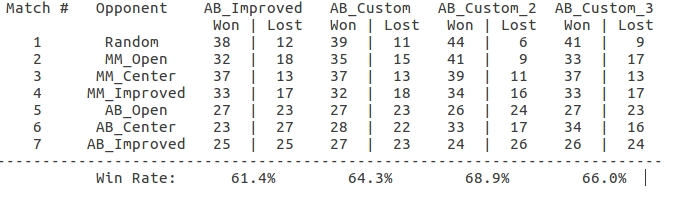
\includegraphics[scale=1]{isolation_results.jpg}

All the heuristics have been evaluated in 50 matches where the first two movements were placed randomly. \newline

The results show that all our agents have beaten the agent ID improved in the total percentage.\newline

The agent that showed a better behavior was the agent AB\_Custom\_2, obtaining a score of $68.9\%$, which corresponds to the heuristic Look ahead improved score v2. In my opinion, the $8\%$ improvement over the AB\_Improved\_ID heuristic is due to the following reasons:

\begin{enumerate}
\item The heuristic performs a lightweight lookahead of 3 positions which allow us to overcome the problem that a position with more moves can result in positions with fewer moves (As explained in Open move score).

\item The heuristic encourages the positions in open areas. As we perform a look ahead of 3 positions, we will be able to reach open areas 2 steps back.

\item We are taking in account the moves of the opponent, so the heuristic also tries to minimize the number of moves of the opponent. (We utilize a lookahead of 3 positions as well)
\end{enumerate}
\end{document}
